\documentclass[times, utf8, diplomski]{fer}
\usepackage{booktabs}
\usepackage{cite}
\usepackage{graphicx}
\usepackage{xcolor}
\usepackage[]{algorithm2e}
\usepackage{bbm}
\usepackage{multirow}
\usepackage{float}

\graphicspath{ {./img/} }

% Math
\def\mat#1{\underline{#1}}
\def\expect{\mathbb{E}}
\def\realnum{\mathbb{R}}
\def\pfrac#1#2{\frac{\partial #1}{\partial #2}}
\def\dfrac#1#2{\frac{d #1}{d #2}}
\def\F1{F$_1$}

% TODO notes
\def\TODO#1{\noindent\textcolor{red}{TODO: \textit{#1}}\newline}
\def\todo#1{\TODO{#1}}
\def\todoimg#1{\begin{center} \textcolor{red}{\big[ IMAGE: \textit{#1} \big]} \end{center}}

\begin{document}

\thesisnumber{1966}

\title{Optimizirane izlazne funkcije klasifikatora temeljenog na umjetnim neuronskim mrežama u domeni implementacijskih napada na kriptografske uređaje}

\author{Juraj Fulir}

\maketitle

% Ispis stranice s napomenom o umetanju izvornika rada. Uklonite naredbu \izvornik ako želite izbaciti tu stranicu.
\izvornik

\zahvala{ZAHVALA'n'STUFF}

\tableofcontents

%--------------------------------------------------------------------------------------%
\chapter{Uvod}
\todo{ Opis problema }

%--------------------------------------------------------------------------------------%
\chapter{Implementacijski napadi na kriptografske uređaje}

\section{Side-channel napadi}
\todo{ Postoji nekoliko vrsta.}
\todo{ Ovdje se obrađuje DPA.}

\section{Izvedba napada}
\todo{ Uštekaj uređaj, osciloskop na to i to mjesto i snimaj}
\todo{ Provjeri mogućnosti i zaključi najvjerojatniju}
\todo{ Problem netraktabilnosti postupka -> neuralke <3}

\section{DPA skupovi podataka}
\todo{Tko i cilj*}
\todo{Ne zaboravi referencu na stranicu!}

\subsection{DPAv2}
\todo{Kada je napravljen i ko ga je radil}
\todo{Jel HW ili onaj pravi}
\todoimg{PCA redukcija iz jn}
\todoimg{Statistike iz jn}
\todo{Mjere dobrote klasifikacije}

\subsection{DPAv4}
\todo{Kada je napravljen i ko ga je radil}
\todo{Jel HW ili onaj pravi}
\todoimg{PCA redukcija iz jn}
\todoimg{Statistike iz jn}
\todo{Mjere dobrote klasifikacije}

%--------------------------------------------------------------------------------------%
\chapter{Klasifikator temeljen na umjetnim neuronskim mrežama}

\section{Umjetne neuronske mreže}
Umjetne neuronske mreže (nadalje „neuronske mreže“) koristimo za modeliranje višedimenzijske funkcije ili distribucije kojom se aproksimira rješenje zadanog problema iz konačnog broja primjera. Vrlo su moćan alat za savladavanje teških zadataka u raznim područjima, često dostižući ljudske performanse na zadanom problemu. Danas su vrlo raširene u raznim područjima od kojih su samo neka: računalni vid \citep{alexnet,yolo}, prirodna obrada jezika \citep{word2vec,char_cnn} i podržano učenje \citep{atari,active_learn}.

\subsection{Građa}
Neuronske mreže građene su od međusobno povezanih jedinica, tzv. neurona, modeliranih prema pojednostavljenom modelu biološkog neurona. Neuron očitava ulazne značajke sustava ili izlaze drugih neurona te ažurira svoje unutarnje stanje (aktivaciju) i stvara odziv (izlaz). Utjecaj ulaza na neuron vrednuje se težinama \engl{weights} koje definiraju kako se neuron ponaša u ovisnosti o pojedinim ulazima. Aktivacijski prag neurona \engl{bias} određuje jedinstvenu osjetljivost neurona na jačinu podražaja. Težine i prag neurona nazivamo parametrima neurona.

\todo{Što sve biolozi vele o neuronima? https://www.ncbi.nlm.nih.gov/pmc/articles/PMC3812748/}

\begin{figure}[h]
\centering
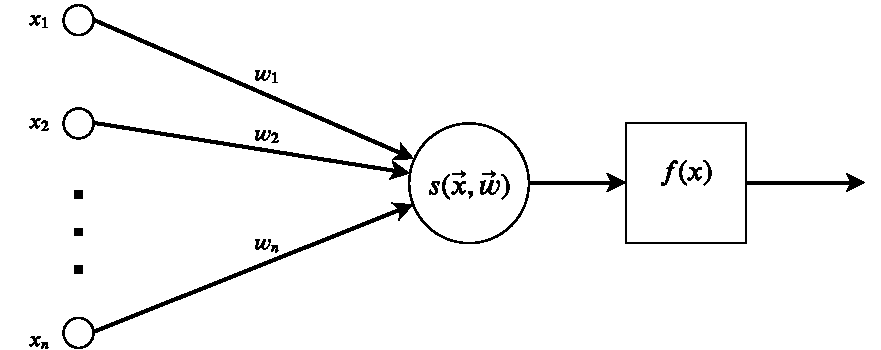
\includegraphics[scale=0.7]{Neuron.pdf}
\caption{Prikazani osnovni dijelovi neurona su težine dendrita ($w_i$), aktivacijska funkcija ($a(\vec{x},\vec{w})$) i izlazna funkcija ($f(x)$). Prag neurona nije prikazan zbog jednostavnosti dijagrama.}
\label{fig:neuron}
\end{figure}

Način na koji iz ulaza gradimo unutarnje stanje (aktivaciju) neurona opisujemo aktivacijskom funkcijom. Najpopularnije aktivacijske funkcije jesu afina funkcija i unakrsna korelacija.
Afina funkcija je skalarni produkt vektora ulaza s vektorom težina neurona uz dodatak vrijednosti praga. Parametri neurona definiraju nagib i pomak ravnine u prostoru ulaza koja opisuje aktivaciju neurona. Primijenjuje se kada se ulazi u model mogu zapisati vektorom značajki čiji raspored nije bitan.
\begin{equation}
f(\vec{x};\mat{W},\vec{b})=\mat{W}^T \cdot \vec{x} + \vec{b}
\end{equation}

\todo{Spomeni distance based aktivacije (ANFIS?)}
\todo{Spomeni i složenije metode: \citep{network_in_network}}

Pretvorbu aktivacije neurona u izlazni signal opisujemo izlaznom funkcijom koja se detaljnije obrađuje u poglavlju \ref{sec:izlazne_fje}. Aktivacijska i izlazna funkcija definiraju prijenosnu funkciju koja ujedno opisuje ponašanje cijelog neurona \citep{function_survey}. U praksi se pojam aktivacijske i prijenosne vrlo često ekvivalentno koristi na mjestu pojma izlazne funkcije, no ovaj rad se drži prethodno navedene i jasnije notacije.
\begin{equation}
t(x) = (f \circ a)(x) = f(a(x))
\end{equation}

Povezivanjem neurona gradi se arhitektura mreže koja određuje kako podatci i gradijenti teku kroz mrežu, a time utječu na brzinu učenja i inferencije neuronske mreže. Najčešće se koriste slojevite unaprijedne arhitekture zbog jednostavnosti izvedbe. Unaprijedne arhitekture propuštaju podatke samo u jednom smjeru odnosno već izračunati neuroni se ne izračunavaju ponovno, što je posebno pogodno za optimizaciju širenjem unatrag, detaljnije opisanu u poglavlju \ref{sec:backprop}. Slojevite arhitekture omogućuju paralelizaciju izvođenja operacija na grafičkim karticama što značajno ubrzava postupke učenja i inferencije. Pri definiciji slojevite arhitekture najčešće je dovoljno navesti samo redoslijed slojeva, no ponekad je potrebno definirati i način povezivanja slojeva npr. pri uporabi preskočnih veza \citep{highwaynet, resnet, densenet}. Prvi sloj služi za postavljanje ulaza mreže i nazivamo ga ulaznim slojem mreže. Posljednji sloj mreže služi nam za ekstrakciju izlaza te mjerenje kakvoće mreže i nazivamo ga izlaznim slojem mreže. Svi slojevi između ulaznog i izlaznog sloja nazivaju se skrivenim slojevima.

Potpuno povezana arhitektura je najjednostavnija arhitektura za zadatak klasifikacije. Svaki neuron u potpuno povezanom sloju aktivira se pomoću svih izlaza iz prethodnog sloja. Za naučeni potpuno povezani sloj kažemo da vrši ekstrakciju značajki iz svojih ulaza. Geometrijski gledano, svaki neuron vrši mapiranje značajki iz dimenzije prethodnog sloja u novu dimenziju s ciljem modeliranja boljih značajki.

\todo{Daj neki dokaz za ovo gore.}

Unakrsna korelacija, za razliku od afine funkcije, koristi informaciju o susjednosti ulaznih značajki. Ulaz za takav model je definiran n-dimenzijskim tenzorom, a neuron uzima samo jedan pod-tenzor ulaza (vidljiva regija) i nad njime računa skalarni produkt s n-dimenzijskim tenzorom parametara (jezgrom). Kada su ulazi slike u boji ulazni tenzor ima 3 dimenzije (visina, širina, RGB kanali) pa stoga i jezgra ima 3 dimenzije, no znantno manje visine i širine. Unakrsna korelacija prozvana je konvolucijom jer radi na istom principu, a jedina razlika je da se elementi jezgre indeksiraju zrcaljeno po obje osi. S obzirom da se parametri jezgre uče automatski, nije nam bitno definirati orijentaciju jezgre.
\begin{equation}
f(\mat{X};\mat{W})=\mat{X} \circledast \mat{W}
\end{equation}

\todo{Je li uopće potrebno spominjat konvoluciju?}
\todo{Raspisat konvoluciju po elementima?}

\subsection{Optimizacija umjetne neuronske mreže}
Optimizacijom parametara neuronska mreža prilagođava se danom zadatku, odnosno kažemo da mreža 'uči'. Optimizaciju parametara najčešće izvodimo gradijentnim spustom, uz pretpostavku derivabilnosti svih komponenata neuronske mreže. Kada ta pretpostavka ne vrijedi koriste se algoritmi kombinatorne optimizacije poput evolucijskih algoritama. U ovom radu optimizacija se vrši gradijentnim spustom.

\subsubsection{Gradijentni spust}
\label{sec:gradijentni_spust}

\todoimg{gradijentni spust unimodalna vs višemodalna (gdje preskoći brdo i uleti u bolji optimum)}
\label{fig:gradientni_spust}

Gradijentni spust je algoritam pronalaska minimuma funkcije vođen gradijentom te funkcije. Za zadanu početnu točku iterativno se pomiče u smjeru suprotnom od gradijenta funkcije u toj točki dok ne zadovolji neki od uvijeta zaustavljanja. Na strmim funkcijama gradijent je često prevelik i može izazvati oscilaciju ili divergenciju (slika \ref{fig:oscilira_divergira}). Stoga se gradijent pri pomaku skalira koeficijentom pomaka $\mu$. Dobro odabran koeficijent pomaka može osigurati bržu konvergenciju, a kod višemodalnih funkcija i pronalazak boljeg optimuma (slika \ref{fig:gradientni_spust}).

Početna točka utječe na ishod algoritma. Kod višemodalnih funkcija s optimumima različitih kvaliteta, početna točka može definirati u koji će lokalni optimum algoritam konvergirati (slika \ref{fig:pocetna_tocka}). 

\begin{algorithm}[H]
\KwIn{funkcija $f(\vec{x})$}
\KwIn{početna točka $\vec{x_0}$}
\KwIn{koeficijent pomaka $\eta$}
\KwIn{broj iteracija $n$}
\For{n iteracija}{
$\vec{g_i} \gets \vec{\nabla}_{\vec{x}} f(\vec{x_i})$ \;
$\vec{x_{i+1}} \gets \vec{x_i} - \eta \cdot \vec{g_i}$
}
\KwResult{konačna točka $\vec{x_i}$ je pronađeni optimum}
\caption{Gradijentni spust}
\label{alg:grad_spust}
\end{algorithm}

\todoimg{graidjentni spust stope spuštanja (velka, mala, taman)}
\label{fig:oscilira_divergira}

Broj iteracija definira koliko se puta pomičemo iz početne točke, što definira i trajanje algoritma. Generalno želimo skratiti vrijeme pretraživanja te povećati koeficijent spusta kako bismo koristili manje pomaka. No u praksi najčešće nailazimo na višemodalne funkcije sa strmim regijama koje izazivaju oscilacije i mogu izazvati divergenciju. Stoga se češće koriste manji pomaci kroz više iteracija. Dodatno se mogu dodati modifikacije gradijenta koje nude ograničavaju veličinu gradijenta (odsijecanje gradijenta i sl.).

\todoimg{gradijentni spust sa početnim točkama (jedna ode u lok, jedna ode u glob, jedna zapne desno na platou)}
\label{fig:pocetna_tocka}

Problem se javlja ako algoritam "odluta" u visoravan na kojoj su gradijenti vrlo mali, a sama regija je s obzirom na pomake ogromna (slika \ref{fig:pocetna_tocka}). Kad gradijent postane neupotrebljivo malen kažemo da je "\textit{iščeznuo}". U takvim slučajevima pomaže dodavanje momenta koji se akumulira kroz više iteracija i dodaje vektoru gradijenta. Kad algoritam naiđe na regiju s vrlo malim gradijentima, moment pokušava izvuči algoritam iz visoravni pomičući ga u smjeru koji je akumuliran. Kako moment ne bi izvukao algoritam iz optimuma, dodaje mu se koeficijent "\textit{zaboravljanja}" kojim se stari vektor momenta djelomično zaboravlja u korist novog vektora pomaka (jednadžba \ref{eq:moment_update}). Moment može pomoći i pri zaobilaženju lokalnih optimuma (slika \ref{fig:pocetna_tocka}).

\begin{equation}
\label{eq:moment_update}
\begin{split}
\vec{v} &\gets \alpha \cdot \vec{v} - \eta \cdot \vec{g} \\
\vec{x} &\gets \vec{x} + \vec{v}
\end{split}
\end{equation}

\todoimg{moment prije i na visoravni, moment za savladavanje brda}
\label{fig:visoravan}

Algoritam je primijenjiv na funkcije proizvoljne dimenzionalnosti uz pretpostavku derivabilnosti u svakoj točki. Za proizvoljnu realnu funkciju, uz dobro odabrane hiperparametre, algoritam će konvergirati u jedan od lokalnih optimuma, no algoritam generalno nema garanciju konvergencije u globalni optimum. Garanciju pronalaska globalnog optimuma nudi jedino za trivijalne unimodalne funkcije uz odgovarajuće hiperparametre algoritma (slika \ref{fig:gradientni_spust}).

Problem odabira hiperparametara proizlazi iz činjenice da u generalno praksi nemamo definiranu funkciju koju minimiziramo (već samo skup primjera te funkcije) i/ili ju ne možemo jasno vizualizirati (kada radimo s funkcijama visoke dimenzionalnosti). Čak i da imamo definiranu funkciju najčešće ne znamo koju vrijednost poprima globalni optimum, a pohlepna pretraga je netraktabilna. Unatoč tome, gradijentni spust efikasno i učinkovito pronalazi optimume koji su dovoljno dobri za većinu praktičnih primjena \citep{yolo}.

\subsubsection{Funkcija gubitka}
Pri učenju umjetnih neuronskih mreža potrebno je definirati funkciju gubitka. Funkcija gubitka, za dani ulaz, uspoređuje predikciju mreže sa željenim vrijednostima te dodjeljuje iznos pogreške (realan broj). Potrebno je pažljivo odabrati funkciju gubitka jer utječe na učenje svakog parametra (kao što je opisano u poglavlju \ref{sec:backprop}) te definira što je ishod učenja. 

Najčešće ne znamo definiciju funkcije gubitka na čitavoj promatranoj domeni već posjedujemo samo uzorke te funkcije u podatcima koje smo izmjerili i koje smatramo reprezentativnim. Ovdje pretpostavljamo da će neuronska mreža ostvariti svojstvo generalizacije, koje je detaljnije objašnjeno u poglavlju \ref{sec:svojstva}. Stoga se u narednim formulama koristi notacija sumiranja.

Funkcija gubitka često je usko vezana uz vrstu problema koji se rješava (klasifikacija, regresija i ostali), način učenja (nadzirano, polu-nadzirano, nenadzirano, podržano) i izlaznu funkciju posljednjeg sloja neuronske mreže. U ovom radu vrši se klasifikacija nadziranim učenjem, no u nastavku se navodi i primjer funkcije gubitka za regresiju.

Uobičajeno se za funkciju gubitka koristi negativna logaritamska izglednost ...

\todo{oba imaju neg.log.izglednost, no pretpostavljaju razl. distribucije da dobiješ kvadratni (gauss) ili ovaj drugi loss (kategorička ilitiga Bernoullijeva)}

U problemima regresije, najčešće se koristi funkcija kvadratnog gubitka koja računa odstupanje izlaza neuronske mreže od željenih vrijednosti. Uz ovaj gubitak najčešće se koristi funkcija identiteta u izlaznom sloju. Ova funkcija je brza i jednostavna
\begin{equation}
\label{eq:loss_regression}
L(\theta) = \expect_{(\vec{x},\vec{y})\in (X,Y)???} \sum_{i}^{|\vec{y}|} (f(\vec{x};\theta)_i - \vec{y}_i)^2
\end{equation}

U problemima klasifikacije, koristi se funkcija negativne logaritamske izglednosti. 
\begin{equation}
\label{eq:loss_classification}
L(\theta) = -\expect ...
\end{equation}

\todo{prebaci očekivanja u SGD, ovdje spomeni samo fje gubitka}

\subsubsection{Optimizacija širenjem unatrag}
\label{sec:backprop}
Funkcija gubitka opisuje pogrešku čitave mreže te ovisi o svakom ugodljivom parametru mreže. Takva formulacija problema omogućuje nam da svaki parametrar mreže ugađamo gradijentnim spustom. Dakle, za parametriziranu funkciju $f(x;\theta)$ tražimo one parametre $\theta^*$ za koje je gubitak najmanji na danim parovima ulaznih i izlaznih podataka.
\begin{equation}
\theta^* = argmin_\theta L(x,y; \theta), \quad \forall (x,y) \in (X,Y)
\end{equation}

Optimiranje gradijentnim spustom zahtjeva derivabilnost funkcije koju optimiziramo po ulazima, što izrazi \eqref{eq:loss_regression} i \eqref{eq:loss_classification} zadovoljavaju. Pri tome koristi se pravilo ulančavanja parcijalne derivacije kompozicije funkcija.
\begin{equation}
\dfrac{}{x} f(g(x)) = \pfrac{f(g(x))}{g(x)} \cdot \pfrac{g(x)}{x}
\end{equation}

Derivacijom funkcije gubitka za regresiju \eqref{eq:loss_regression} po ulazima, uz pretpostavku derivabilnosti čitave neuronske mreže po ulazima, dobivamo sljedeći izraz:
\begin{equation}
tODO
\end{equation}

S obzirom da se mreža sastoji od ulančanih nelinearnih neurona s parametrima, gradijent gubitka moramo proslijediti sekvencijalno širenjem unazad (prema ulazima u mrežu). Pojedini neuron možemo smatrati parametriziranom funkcijom koju je moguće prikazati grafom \ref{fig:neuron_grad}. Vidimo da se ulazni gradijent prolaskom kroz neuron širi na ostale elemente i na ulaze neurona koji vode do prethodnih neurona. Primijetimo i da se širi u suprotnom smjeru od toka podataka. Iz toga proizlazi naziv "\textit{širenjem unazad}" \engl{backpropagation}.

\todoimg{neuron kao graf + tok gradijenata}
\label{fig:neuron_grad}

Želimo li učiti mrežu gradijentnim spustom, svaki parametar mreže treba imati pristup gradijentu funkcije gubitka. S obzirom da je neuron parametrizirana funkcija, pomoću koje ulančavanjem gradimo mrežu, dovoljno je pokazati da pojedini neuron osigurava svojim parametrima pristup gradijentu te da gradijent šalje svojim prethodnicima s kojima je povezan. Na slici \ref{fig:neuron_grad} vidimo da je to ostvarivo, što dokazuju i izrazi:
\begin{align}
\begin{split}
\pfrac{L(x,y;\theta)}{s(x;w)} &= \pfrac{L(x,y;\theta)}{o(x;w)} \cdot \pfrac{o(x;w)}{s(x;w)} \\
&= \pfrac{L(x,y;\theta)}{o(x;w)} \cdot f'(x)
\end{split}
\end{align}

\begin{align}
\begin{split}
\pfrac{L(x,y;\theta)}{x_i} &= \pfrac{L(x,y;\theta)}{s(x;w)} \cdot \pfrac{s(x;w)}{x_i} \\
&= \pfrac{L(x,y;\theta)}{o(x;w)} \cdot f'(x) \cdot w_i
\end{split}
\end{align}

\begin{align} \label{eq:w_update}
\begin{split}
\pfrac{L(x,y;\theta)}{w_i} &= \pfrac{L(x,y;\theta)}{s(x;w)} \cdot \pfrac{s(x;w)}{w_i} \\
&= \pfrac{L(x,y;\theta)}{o(x;w)} \cdot f'(x) \cdot x_i
\end{split}
\end{align}

\begin{align}
\begin{split}
\pfrac{L(x,y;\theta)}{w_0} &= \pfrac{L(x,y;\theta)}{s(x;w)} \cdot \pfrac{s(x;w)}{w_0} \\
&= \pfrac{L(x,y;\theta)}{o(x;w)} \cdot f'(x) \cdot 1
\end{split}
\end{align}

\subsubsection{Stohastički gradijentni spust}

\todo{ne možemo čitav ds odjednom jer je prevelik}
\todo{ne možemo stohastički jer je prešumovito, a i skupo na gpu}
\todo{all hail the mini-batch, aproksimacija taman šumovita da pomaže, spomeni usrednjavanje gradijenta po batchu}
\todo{može i sampliranjem, ali ako imamo dataset kako znamo koliko koje semplirat -> bolje po epohama}
\todo{algoritam SGD}

\subsubsection{Optimizator}
U prethodnim poglavljima opisan je postupak stohastičkog gradijentnog spusta i definicije gradijenta po parametrima, koji su potrebni za ispravno računanje

\todo{uporaba momenta i momenta na kvadrat (interpretacija)}
\todo{Adam}
\todo{smanjivanje stope učenja}

\subsubsection{Promijenjiva stopa učenja}
\todo{zbog nekonveksnih izbočina tam dolje, stopa može biti prejaka}
\todoimg{konveksasta fja u kojoj skok u višljim regijama stvara manje problema od skokova u nižim}

\todo{koristim step reduction}
\todo{postoji množenje faktorom pri detekciji konvergencije, ali ne želim ga jer ne znam kada konvergira (stepeničasto učenje)}

\subsubsection{Inicijalizacija parametara}
Inicijalizacija parametara mreže je sinonim za odabir početne točke pri gradijentnom spustu.

\todo{važnost dobre inicijalizacije}
\todo{Xavier}

\subsection{Regularizacija}
\label{sec:regularizacija}
\todo{geometrijski opis deciziske granice}
\todo{podnaučena, generalizira, prenaučena}
\todoimg{podnaučena, generalizira, prenaučena}

\paragraph{Regularizacija parametara}
\todo{L1}
\todo{L2}
\todo{Spomeni pokoju još (adversarial iz Hintona, one za style transfer, ...)}

\paragraph{Regularizacija šumom}
\todo{inherentno zbog šumovitih ulaznih podataka}
\todo{može povećati dataset}

\subsection{Odabir hiperparametara}
Do ovdje su navedeni hiperparametri koji se koriste pri spomenutim tehnikama optimizacije neuronske mreže (poglavlja \ref{sec:gradijentni_spust} - \ref{sec:regularizacija}). No neuronska mreža ima i strukturalne hiperparametre.

Arhitektura mreže je vrlo bitan hiperparametar koji određuje složenost modela te utječe na brzinu inferencije i učenja modela. Razvijene su razne arhitekture koje koriste preskočne veze za postizanje vrlo dubokih arhitektura \citep{resnet, densenet}. Preskočne veze omogućavaju direktniji prijenos gradijenta što pomaže kod problema iščezavajućeg gradijenta u dubokim mrežama (poglavlje \ref{sec:iscezavajuci_grad}). Arhitektura može omogućiti dodatnu paralelizaciju inferencije i učenja tako da se teške operacije raspodijele na više uređaja, a rezultati spoje samo kada je to nužno \citep{alexnet}.

\todo{Izlazne funkcije}

\subsubsection{Procjena generalizacije i odabir modela}
Skup podataka kojim učimo model najčešće ne opisuje stvarnu funkciju potpuno, već sadrži primjere koje smatramo reprezentativnim i koji su dovoljni za njeno modeliranje. Kako bismo procjenili koliko dobro naš model procjenjuje stvarnu funkciju ispitujemo model na podatcima koji nisu korišteni prilikom učenja, odnosno na neviđenim podatcima. Ta se metoda zove \textbf{unakrsna validacija}, a skupove nazivamo \textbf{skupom za učenje} i \textbf{skupom za testiranje}. Dakako, važno je pobrinuti se da su oba skupa reprezentativna stvarnoj funkciji, ali da ne sadrže iste primjere. U suprotnom mreža će naučiti pogrešnu funkciju što može dati lažno pesimistične rezultate ili ćemo nepotpuno ili pristrano testirati što može dovesti do lažno optimističnih rezultata.

Svojstvo modela da dobro modelira na neviđenim primjerima naziva se generalizacija i detaljnije je opisano u poglavlju \ref{sec:generalizacija}. Pri odabiru hiperparametara ili pri odabiru modela potrebno je usporediti generalizaciju svakog pomoću zajedničke mjere. U problemima regresije najčešće se koristi ukupna vrijednost funkcije gubitka na čitavom skupu za testiranje.

\begin{equation}
\label{eq:mat_zabune_bin}
\begin{tabular}{|c|c|c|} \hline
\large{$_{\hat{y}} \setminus ^y$} & $\top$ & $\bot$ \\ \hline
$\top$	& TP & FP \\ \hline
$\bot$	& FN & TN \\ \hline
\end{tabular}
\end{equation}

Pri \textbf{binarnoj klasifikaciji} definiramo \textbf{matricu zabune} \eqref{eq:mat_zabune_bin} koja sadrži četiri elementa \eqref{eq:true_groups} koji definiraju vrstu pogodka i pogreške.
\begin{align}
\label{eq:true_groups}
\begin{split}
\text{Stvarno pozitivni:} \quad TP &= \sum_{(x,y)\in\mathbb{D}} \mathbbm{1} \{h(x) = \top \wedge y = \top \} \\
\text{Stvarno negativni:} \quad TN &= \sum_{(x,y)\in\mathbb{D}} \mathbbm{1} \{h(x) = \bot \wedge y = \bot \} \\
\text{Lažno pozitivni:}   \quad FP &= \sum_{(x,y)\in\mathbb{D}} \mathbbm{1} \{h(x) = \top \wedge y = \bot \} \\
\text{Lažno negativni:}   \quad FN &= \sum_{(x,y)\in\mathbb{D}} \mathbbm{1} \{h(x) = \bot \wedge y = \top \}
\end{split}
\end{align}

Iz tih skupova tada gradimo složenije mjere. \textbf{Točnost} je mjera kojom iskazujemo postotak točno pogođenih primjera:
\begin{equation}
Acc = \frac{TP+TN}{TP+TN+FP+FN}
\end{equation}

Točnost je dobra mjera, no samo ako je brojnost klasa u podatkovnom skupu balansiran. Ako je brojnost jedne klase puno veća od druge tada će trivijalan klasifikator, koji sve primjere klasificira u tu klasu, davati veliku točnost i razlika naspram ispravnijeg klasifikatora biti će nezamjetna. Stoga se kod nebalansiranih setova češće koristi \textbf{\F1 mjera}, koja uzima u obzir \textbf{preciznost} klasifikatora u razlikovanju pozitivnih primjera od negativnih \eqref{eq:precision} i njegov \textbf{odziv} odnosno obuhvat svih pozitivnih primjera testnog skupa \eqref{eq:recall}. \F1 mjera je definirana kao hamonijska sredina između preciznosti i odziva \eqref{eq:f_measure}. Postoji i generalizirana mjera F$_\beta$ koja dodjeljuje veću težinu preciznosti ili odzivu \eqref{eq:f_beta}, no u ovom radu koristi se samo \F1 koja pridijeljuje jednaku težinu. Harmonijska sredina se koristi jer je najstroža između Pitagorinih mjera za sredinu kao što prokazuje slika \ref{fig:sredine}.
\begin{align}
\text{Preciznost:} \quad P &= \frac{TP}{TP+FP} \label{eq:precision} \\
\text{Odziv:} \quad R &= \frac{TP}{TP+FN} \label{eq:recall} \\
\text{F}_1: \quad F_1 &= 2 \cdot \frac{P \cdot R}{P + R} \label{eq:f_measure} \\
\text{F}_\beta: \quad F_\beta &= (1 + \beta^2) \cdot \frac{P \cdot R}{\beta ^2 \cdot P + R} \label{eq:f_beta}
\end{align}

\begin{figure}[h]
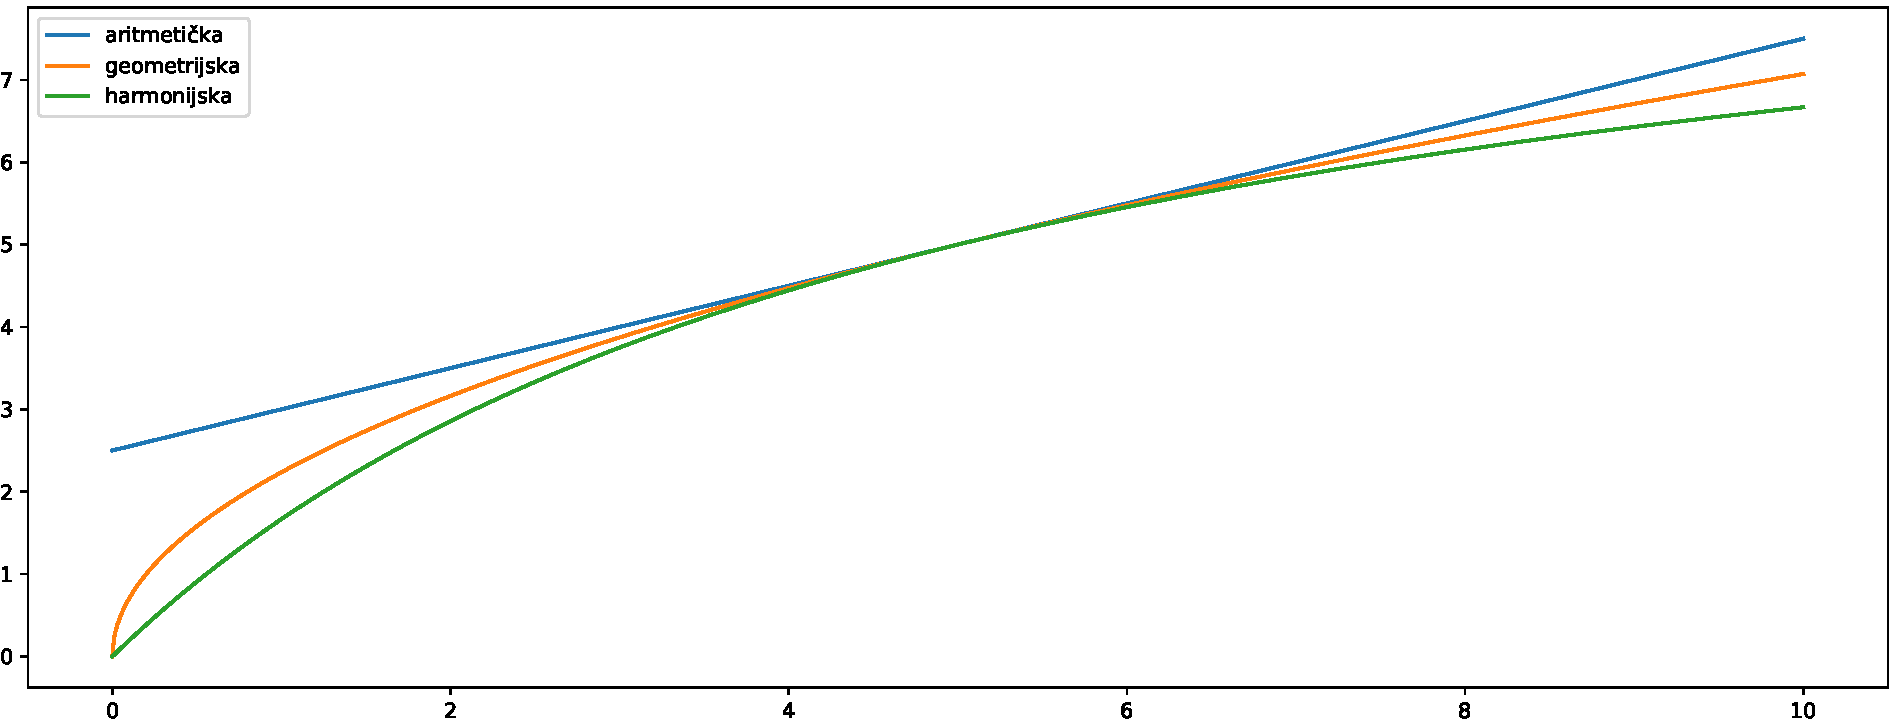
\includegraphics[width=\textwidth]{Pitagorine_sredine.pdf}
\centering
\caption{Pitagorine mjere za sredinu između dviju vrijednosti}
\label{fig:sredine}
\end{figure}

Mjere binarne klasifikacije možemo primijeniti pri \textbf{višeklasnoj klasifikaciji}, no matrica zabune je dimenzija $C\times C$ gdje je $C$ broj klasa. Elementi matrice računaju se slično kao i kod binarne klasifikacije, ali za svaku klasu posebno.
\begin{align}
\label{eq:true_groups}
\begin{split}
\text{Stvarno pozitivni:} \quad TP_i &= \sum_{(x,y)\in\mathbb{D}} \mathbbm{1} \{h(x) =  C_i \wedge y = C_i \} \\
\text{Stvarno negativni:} \quad TN_i &= \sum_{(x,y)\in\mathbb{D}} \mathbbm{1} \{h(x) \neq C_i \wedge y \neq C_i \} \\
\text{Lažno pozitivni:} \quad FP_i &= \sum_{(x,y)\in\mathbb{D}} \mathbbm{1} \{h(x) = C_i \wedge y \neq C_i \} \\
\text{Lažno negativni:} \quad FN_i &= \sum_{(x,y)\in\mathbb{D}} \mathbbm{1} \{h(x) \neq C_i \wedge y = C_i \}
\end{split}
\end{align}

Za izračun složenijih mjera poput točnosti i \F1 mjere moramo računati prosjek po klasama. Razlikujemo dva pristupa računanju prosjeka: makro i mikro. \textbf{Makro prosjekom} se prvo izračunaju mjere svake klase naspram svih ostalih te se uzme njihov prosjek. Ova mjera pretpostavlja jednak utjecaj svih klasa nez obzira na njihovu veličinu \citep{ml_probabilistic}.
\begin{equation}
\begin{split}
Acc^M = \sum_{i=1}^K \frac{Acc_i}{K}
\end{split} \quad
\begin{split}
P^M = \sum_{i=1}^K \frac{P_i}{K}
\end{split} \quad
\begin{split}
R^M = \sum_{i=1}^K \frac{R_i}{K}
\end{split} \quad
\begin{split}
F_1^M = \sum_{i=1}^K \frac{F_{1;i}}{K}
\end{split}
\end{equation}

\textbf{Mikro prosjekom} se prvo zbroje matrice zabune po pojedinim klasama, a zatim se nad zbrojenom matricom računaju mjere. Na mikro prosjek više utječe veličina klasa i koristi se u nebalansiranim skupovima.

\begin{align}
\begin{split}
Acc^\mu &= \frac{\sum_i (TP_i+TN_i)}{\sum_i (TP_i+TN_i+FP_i+FN_i)} = Acc^M \\
FP = FN \implies P^\mu &= R^\mu = F_1^\mu = \frac{\sum_i TP_i}{\sum_i (TP_i+FP_i)}
\end{split}
\end{align}

\subsubsection{Pretraživanje po rešetci}
Najjednostavniji način za pretraživanje hiperparametara je pretraživanje po rešetci. Za svaki hiperparametar koji optimiziramo definiramo vrijednosti koje želimo ispitati. Algoritam tada evaluira dani model za svaku kombinaciju hiperparametara i vraća kombinaciju ili model koji ostvaruje najbolje rezultate.

Iako se optimalni hipermarametri mogu nalaziti izvan zadanih skupova i neće biti pronađeni, postupak je brz i daje dovoljno dobre rezultate za praktičnu primjenu. Često je dovoljno da pronađe kombinaciju hiperparametara za koju model ne divergira niti prestaje učiti određen broj iteracija.

\subsection{Svojstva}
\label{sec:svojstva}

\subsubsection{Univerzalna aproksimacija}
Teorem univerzalne aproksimacije tvrdi da unaprijedna neuronska mreža može modelirati proizvoljnu Borel mjerljivu funkcju proizvoljno dobro uz nekoliko uvijeta: mora imati linearni izlaz, barem jedan nelinearni skriveni sloj koji koristi sažimajuću funkciju i "dovoljan" broj skrivenih neurona. Dakle, postoji arhitektura i postoje parametri kojima neuronska mreža može modelirati zadani podatkovni skup. No, teorem ne iskazuje kako doći do tih parametara što optimizaciju neuronske mreže čini vrlo teškom. \citep{goodfellowbook}

\subsubsection{Dubina}
Iako je prema teoremu univerzalne aproksimacije dovoljan jedan nelinearni skriveni sloj za predstavljanje proizvoljne Borel mjerljive funkcije, gornja granica veličine tog sloja je eksponencijalno velika naspram broja ulaza što je netraktabilno. Dodavanjem dubine moguće je iskoristiti pravilnosti u funkciji koju aproksimiramo kako bismo smanjili potreban broj neurona. Primjer su funkcije simetrične oko neke osi. Ako skriveni slojevi mreže vrše preklapanje te funkcije preko same sebe, uzastopnim preklapanjem dobiva se sve jednostavnija funkcija. Preklapanje mogu vršiti po-dijelovima-linearne izlazne funkcije poput ReLU i Maxout. Dakako, ne postoji garancija da stvarna funkcija zadovoljava svojstvo simetrije, no u praksi dublje mreže generaliziraju bolje \citep{alexnet, highwaynet, resnet, densenet}. Postoje i druge interpretacije utjecaja dubine, poput svojstva dekompozicije zadatka na manje cjeline ili interpretacija neuronske mreže ako računalnog programa koje nadilaze temu ovog rada \citep{goodfellowbook}.

\todo{VC dimenzija}

\subsubsection{Kompresija}
\todo{kompresija}
\todo{https://www.quantamagazine.org/new-theory-cracks-open-the-black-box-of-deep-learning-20170921/}

\subsubsection{Generalizacija}
\label{sec:generalizacija}
\todoimg{underfit-fit-overfit}
\todo{generalizacija}
\todoimg{train-test U curve}

Ovo je posebno izraženo kod klasifikacije slika gdje za jednu generičku klasu (npr. automobil) postoji neprebrojivo mogućih slika s različitim modelom, bojom ili kutom gledanja automobila. No mi raspolažemo sa svega nekoliko stotina tisuća primjera koje smatramo reprezentativnim za tu klasu i želimo izgraditi klasifikator koji je robustan na većinu perturbacija slike.

\todo{negdje spomeni da su neuralke zapravo vrlo ograničene jer ograničavamo prostor mogućnosti zadavanjem fiksnih izlaznih fja, arhitekture i načina optimizacije (induktivna pristranost ograničavanjem skupa hipoteza). leži negdje između GP i ručno izgrađenih modela (jer je neuralka samo stablo funkcija kao u TF). CGP unosi ograničenje strukture što je bliže neuralki i daje zanimljive rezultate (atari cgp). Čini se da im godi balans između strukture i nasumičnosti.}

\subsection{Problemi}
\subsubsection{Odabir hiperparametara}
\todo{Problem odabira arhitekture, aktivacijske funkcije i hiperparametara}
Arhitektura, prijenosne funkcije i parametri definiraju neuronsku mrežu te njihov odabir značajno utjeće na performanse neuronske mreže. Učenje 

\subsubsection{Isčezavajući gradijent}
\label{sec:iscezavajuci_grad}
\todo{Problem dubokih arhitektura}

\subsubsection{Pretreniranost i neprijateljski primjeri}
\todo{Problem pretreniranosti + neprijateljski primjeri}

Derivabilne neuronske mreže optimiziraju se optimizatorom koji određuje kako se mijenjaju parametri. Za ugađanje parametara najčešće se koristi gradijentni spust, uz pretpostavku derivabilnosti čitave neuronske mreže. Kada pretpostavka ne vrijedi najčešće se koriste evolucijski algoritmi.

\section{Izlazne funkcije}
\label{sec:izlazne_fje}
Izlazna funkcija služi unošenju nelinearnosti u neuronsku mrežu i ima utjecaj na njeno učenje. Prilikom inferencije izlazna funkcija stvara nelinearnosti u decizijskoj granici koje su parametrizirane parametrima neurona na koji se primijenjuje. U slojevitim arhitekturama izlazne funkcije se primijenjuju uzastopno s različitim parametrima i vrše nelinearne projekcije iz jedne dimenzije u drugu.

Prilikom učenja neuronske mreže važan nam je utjecaj derivacije izlazne funkcije na gradijent pri širenju unatrag. Prolaskom unazad gradijent se množi s parametrima slojeva koji se mogu zapisati matricom težina $\mat{W}$. Uzastopnom primijenom matrica težina, ako su loše kondicionirane, može doći do "\textit{isćezavanja}" ili "\textit{eksplozije}" gradijenta.

\todo{Bitka za odabir izlazne fje (nađi onaj rad di pljuje po sigmoidi i relu (elu rad?))}

U nastavku su navedene izlazne funkcije koje je autor pronašao u literaturi i koje su isprobane u ovom radu. Za svaku funkciju napisana je formula i iscrtan izgled funkcije i njene derivacije te navedena neka poznata svojstva.

\subsection{Funkcija identiteta}
\engl{Identity function}

\begin{figure}[H]
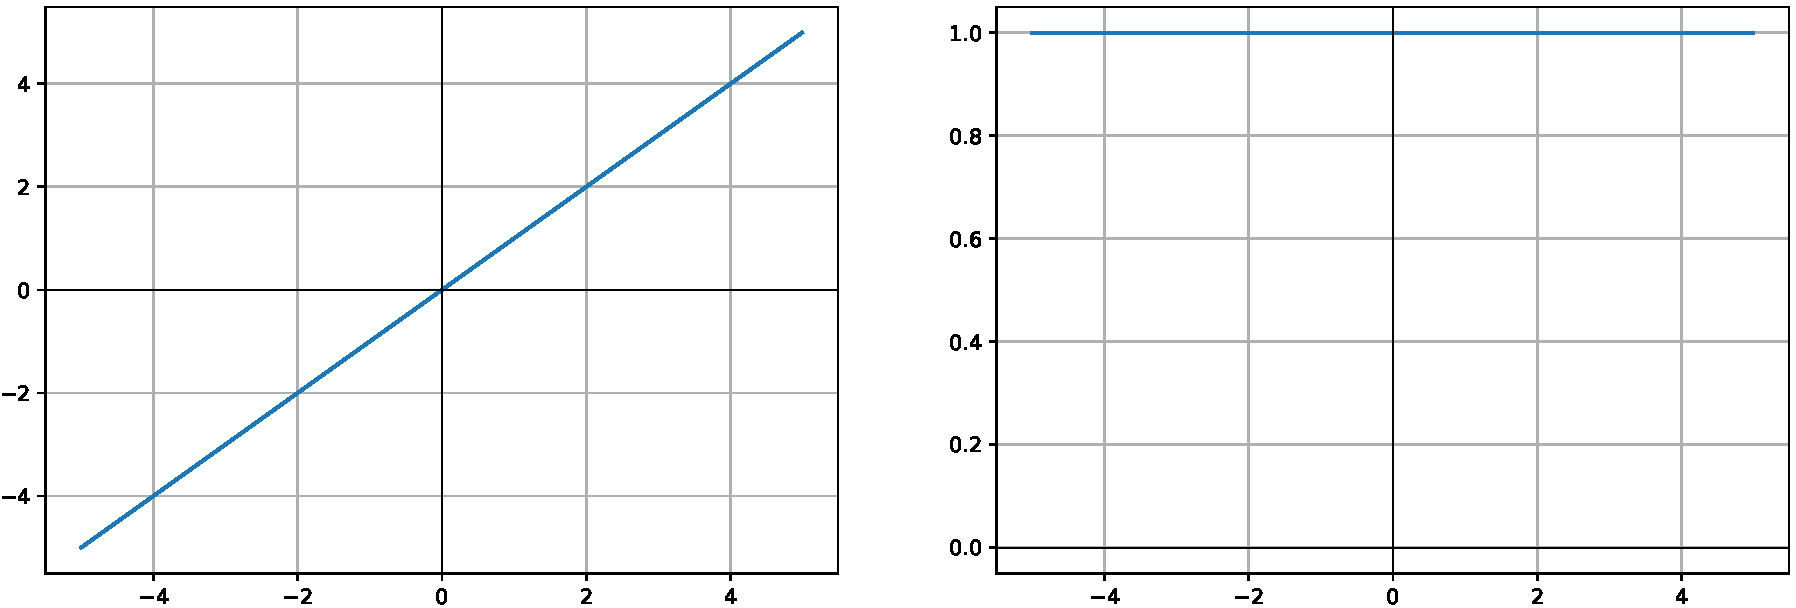
\includegraphics[width=\textwidth]{Identity.pdf}
\centering
\caption{Funkcija identiteta i njena derivacija}
\label{fig:identity}
\end{figure}

\begin{equation}
\begin{split}
f(x) = x
\end{split}
\qquad
\begin{split}
f'(x) = 1
\end{split}
\end{equation}

Funkcija identiteta je jednostavna i brza, no njome neuronska mreža može naučiti samo linearne funkcije. Ako primijenimo funkciju na dva uzastopna sloja vidimo da je konačna funkcija ponovno linearna što znači da ne možemo naučiti mrežu na nelinearnim podatcima:
\begin{align}
\begin{split}
f_l(x) &= w_l \cdot x + b_l \\
f_1(f_2(x)) &= w_1 \cdot (w_2 \cdot x + b_2) + b_1 \\
&= \underline{w_1 \cdot w_2} \cdot x + \underline{w_1 \cdot b_2 + b_1} \\
&= w_{1,2} \cdot x + b_{1,2}
\end{split}
\end{align}

\subsection*{Ispravljena linearna jedinica (ReLU)}
\engl{Rectified linear unit}

\begin{figure}[H]
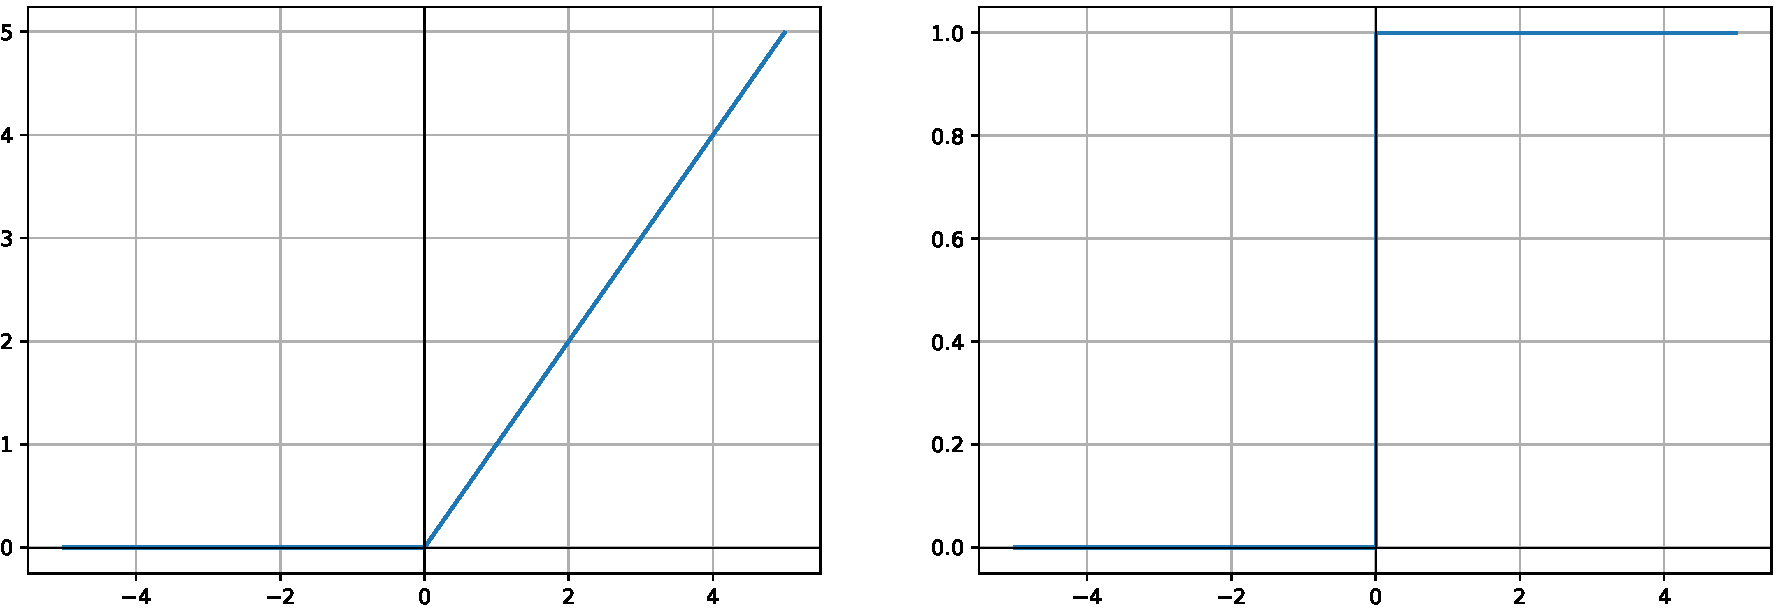
\includegraphics[width=\textwidth]{ReLU.pdf}
\centering
\caption{Funkcija ReLU i njena derivacija}
\label{fig:relu}
\end{figure}

\begin{equation}
\begin{split}
f(x) = 
\begin{cases}
x,		& \text{ako } x > 0 \\
0,		& \text{inače}
\end{cases}
\end{split}
\qquad
\begin{split}
f'(x) = 
\begin{cases}
1,		& \text{ako } x > 0 \\
0,		& \text{inače}
\end{cases}
\end{split}
\end{equation}

\todo{bez i sa cutoff}
\todo{mrtvi neuroni}
\todo{i dalje nije loša}

\todo{koji problem rješava}
\todo{svojstva}
\todo{problemi}

\subsection*{Propusna ispravljena linearna jedinica (LReLU)}
\engl{Leaky ReLU}

\begin{figure}[H]
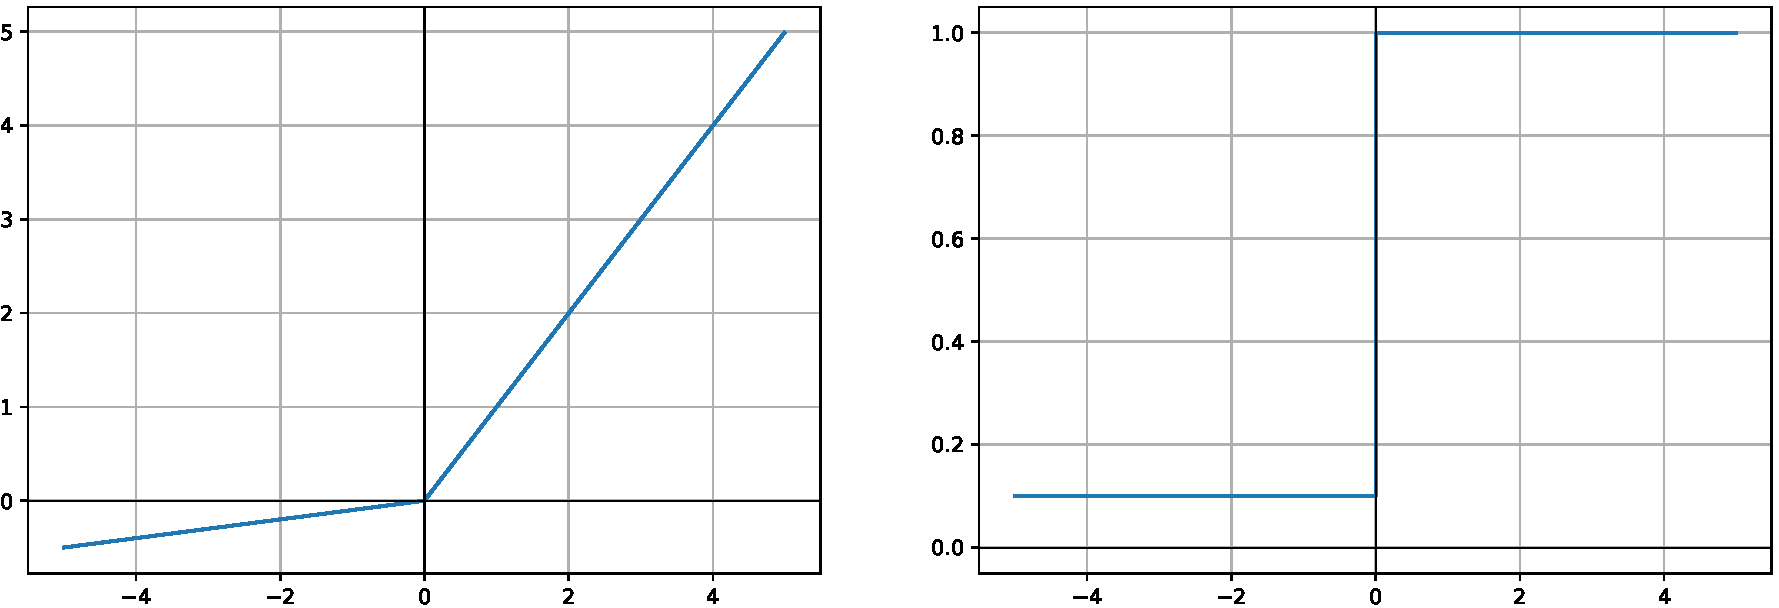
\includegraphics[width=\textwidth]{LReLU.pdf}
\centering
\caption{Funkcija LReLU i njena derivacija za $\alpha=0.1$}
\label{fig:lrelu}
\end{figure}

\begin{equation}
\begin{split}
f(x) = 
\begin{cases}
x,			& \text{ako } x > 0 \\
\alpha x,	& \text{inače}
\end{cases}
\end{split}
\qquad
\begin{split}
f'(x) = 
\begin{cases}
1,		& \text{ako } x > 0 \\
\alpha,	& \text{inače}
\end{cases}
\end{split}
\end{equation}

\todo{koji problem rješava}
\todo{svojstva}
\todo{problemi}

\subsection*{Parametrizirana ispravljena linearna jedinica (PReLU)}
\engl{Parametric ReLU}

\todoimg{}


\begin{equation}
\begin{split}
f(x) &= 
\begin{cases}
x,			& \text{ako } x > 0 \\
\alpha x,	& \text{inače}
\end{cases}
\end{split}
\qquad
\begin{split}
f'(x) = 
\begin{cases}
1,		& \text{ako } x > 0 \\
\alpha,	& \text{inače}
\end{cases}
\end{split}
\end{equation}
\begin{equation*}
\alpha \text{ je učeći parametar}
\end{equation*}

\todo{koji problem rješava}
\todo{svojstva}
\todo{problemi}

\subsection*{Nasumična ispravljena linearna jedinica (RReLU)}
\engl{Randomized leaky ReLU}

\todoimg{}

\begin{equation}
\begin{split}
f(x) &= 
\begin{cases}
x,			& \text{ako } x > 0 \\
\alpha x,	& \text{inače}
\end{cases}
\end{split}
\qquad
\begin{split}
f'(x) = 
\begin{cases}
1,		& \text{ako } x > 0 \\
\alpha,	& \text{inače}
\end{cases}
\end{split}
\end{equation}
\begin{equation}
\alpha \sim U(l,u),\quad l,u \in [0,1]
\end{equation}

\todo{koji problem rješava}
\todo{svojstva}
\todo{problemi}

\subsection*{Ispravljena linearna jedinica s pragom (ThReLU)}
\engl{Thresholded ReLU}

\begin{figure}[H]
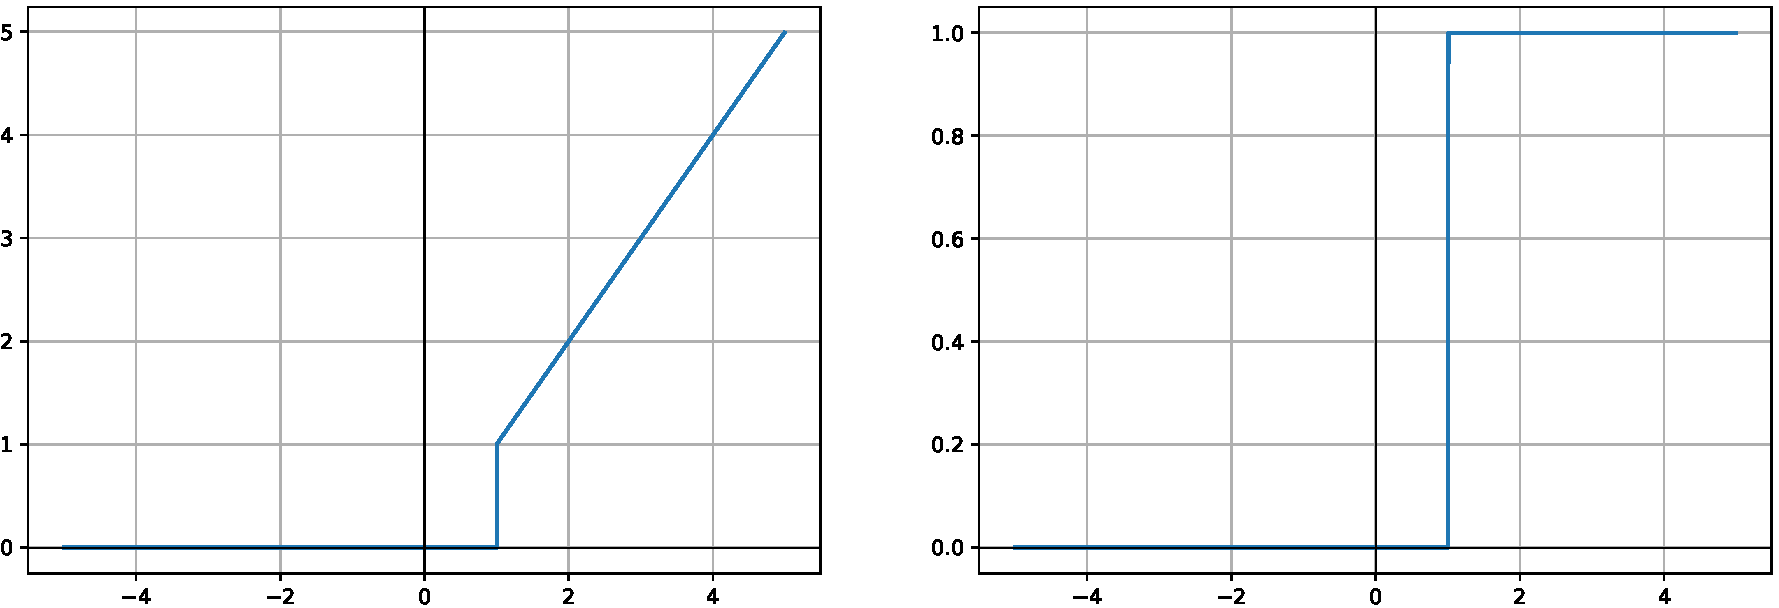
\includegraphics[width=\textwidth]{ThReLU.pdf}
\centering
\caption{Funkcija ThReLU i njena derivacija}
\label{fig:threlu}
\end{figure}

\begin{equation}
\begin{split}
f(x) = 
\begin{cases}
x,		& \text{ako } x > \theta \\
0,		& \text{inače}
\end{cases}
\end{split}
\qquad
\begin{split}
f'(x) = 
\begin{cases}
1,		& \text{ako } x > \theta \\
0,		& \text{inače}
\end{cases}
\end{split}
\end{equation}

\todo{koji problem rješava}
\todo{svojstva}
\todo{problemi}

\subsection*{(DReLU)}
\engl{Dual ReLU}

\todoimg{}

\begin{equation}
???
\end{equation}

\todo{koji problem rješava}
\todo{svojstva}
\todo{problemi}

\subsection*{Eksponencijalno-linearna jedinica (ELU)}
\engl{Exponential linear unit}

\begin{figure}[H]
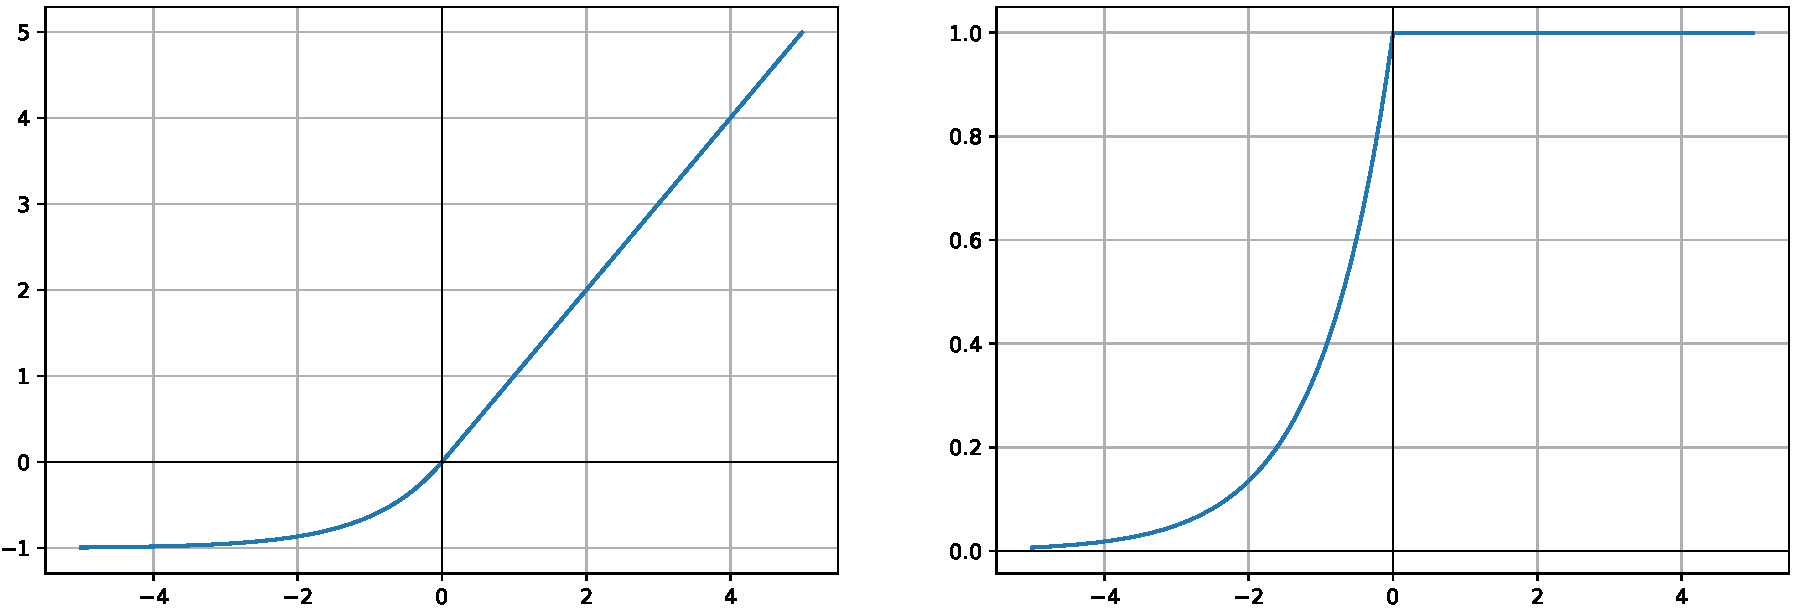
\includegraphics[width=\textwidth]{ELU.pdf}
\centering
\caption{Funkcija ELU i njena derivacija}
\label{fig:elu}
\end{figure}

\begin{equation}
\begin{split}
f(x) = 
\begin{cases}
x,					& \text{ako } x > 0 \\
\alpha (e^x - 1),	&  \text{inače}
\end{cases}
\end{split}
\qquad
\begin{split}
f'(x) = 
\begin{cases}
1,	 		& \text{ako } x > 0 \\
\alpha e^x,	& \text{inače}
\end{cases}
\end{split}
\end{equation}

\todo{koji problem rješava}
\todo{svojstva}
\todo{problemi}

\subsection*{Skalirana eksponencijalno-linearna jedinica (SELU)}
\engl{Scaled exponential linear unit}

\begin{figure}[H]
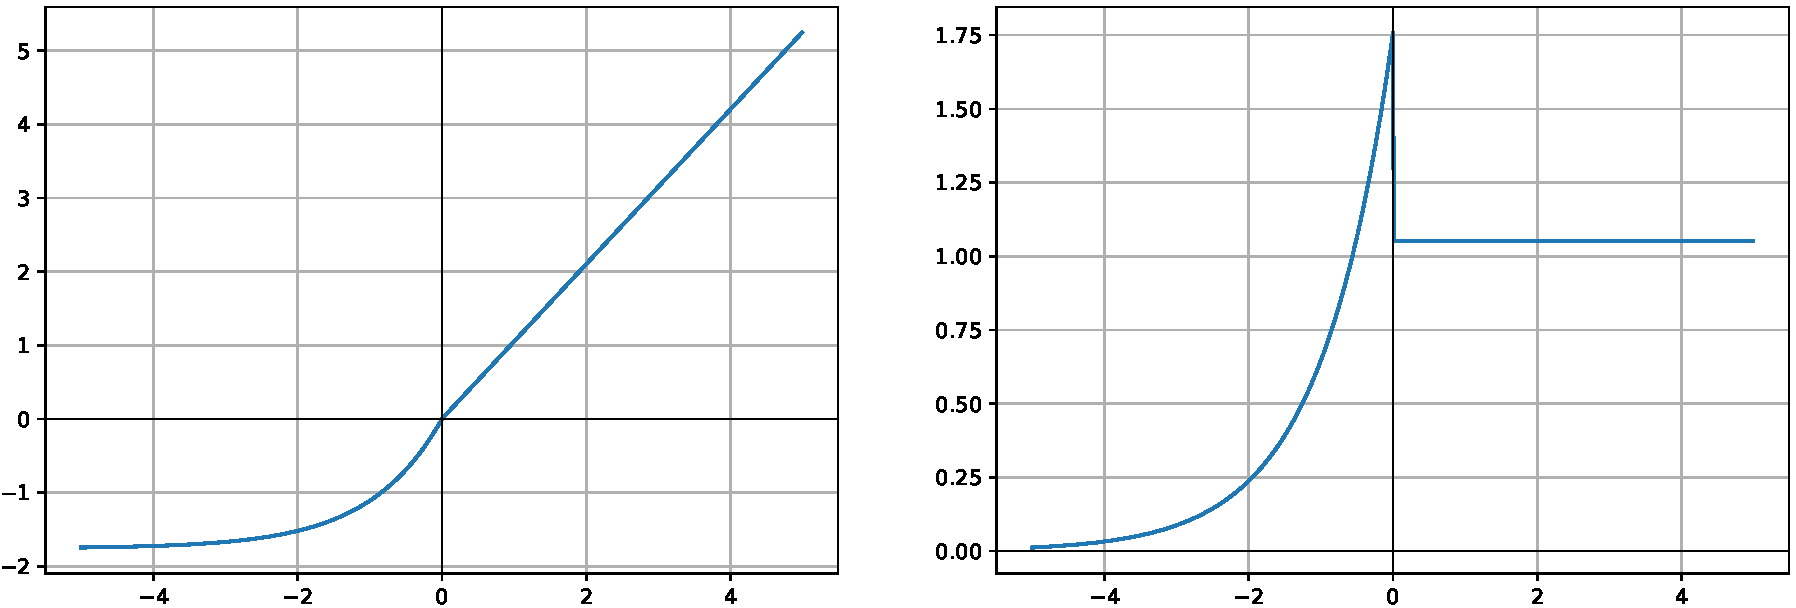
\includegraphics[width=\textwidth]{SELU.pdf}
\centering
\caption{Funkcija SELU i njena derivacija}
\label{fig:selu}
\end{figure}

\begin{equation}
\begin{split}
f(x) = \lambda
\begin{cases}
x,					& \text{ako } x > 0 \\
\alpha (e^x - 1),	&  \text{inače}
\end{cases}
\end{split}
\qquad
\begin{split}
f'(x) = \lambda
\begin{cases}
1,	 		& \text{ako } x > 0 \\
\alpha e^x,	& \text{inače}
\end{cases}
\end{split}
\end{equation}

\todo{koji problem rješava}
\todo{svojstva}
\todo{problemi}

\subsection*{(GELU)}
\engl{Gaussian error linear unit}

\todoimg{}

\todo{koji problem rješava}
\todo{svojstva}
\todo{problemi}

\subsection*{Sigmoida ($\sigma $)}
\engl{Sigmoid}

\begin{figure}[H]
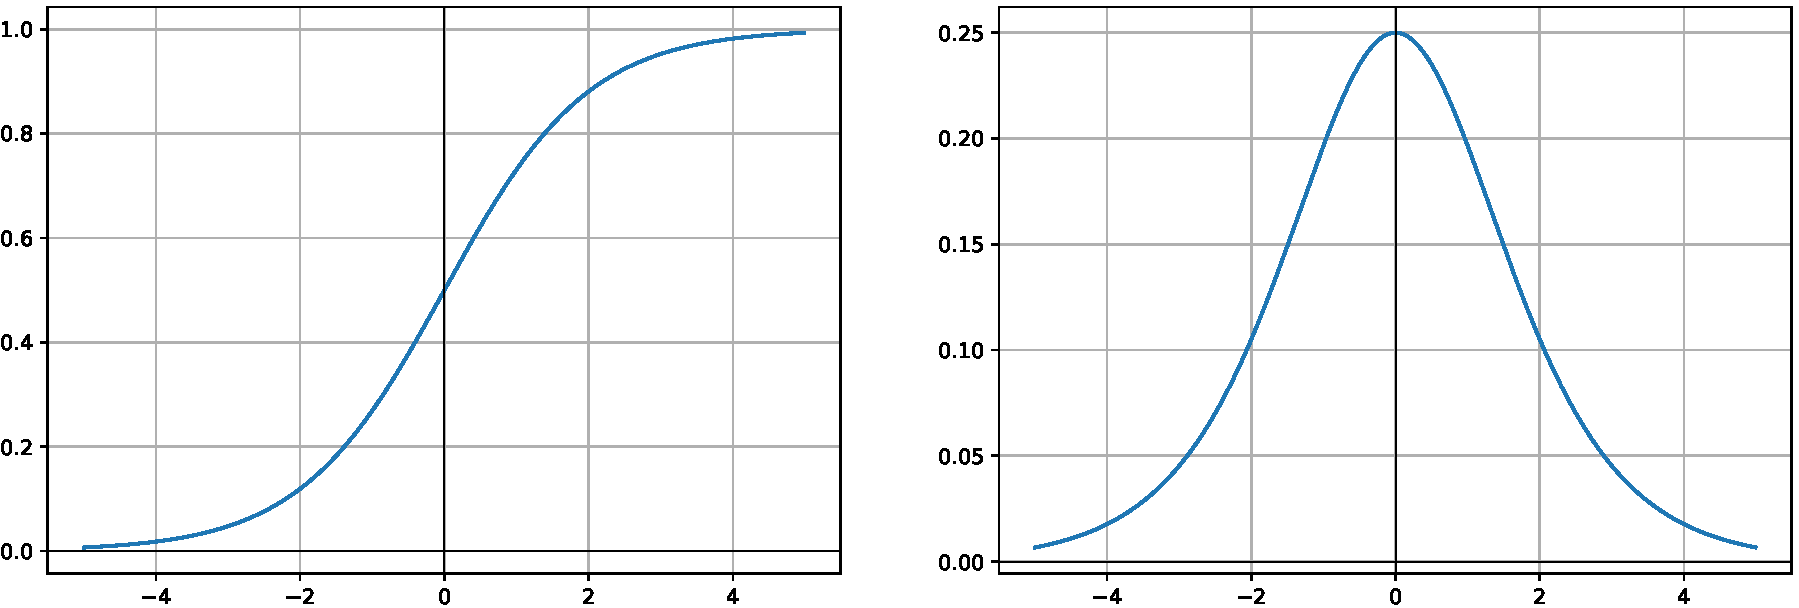
\includegraphics[width=\textwidth]{Sigmoid.pdf}
\centering
\caption{Sigmoida i njena derivacija}
\label{fig:sigmoid}
\end{figure}

\begin{equation}
\begin{split}
f(x) = \frac{1}{1+e^{-x}}
\end{split}
\qquad
\begin{split}
f'(x) = \sigma(x)(1-\sigma(x))
\end{split}
\end{equation}

\todo{koji problem rješava}
\todo{svojstva}
\todo{problemi}

\subsection*{Tvrda sigmoida}
\engl{Hard sigmoid}

\begin{figure}[H]
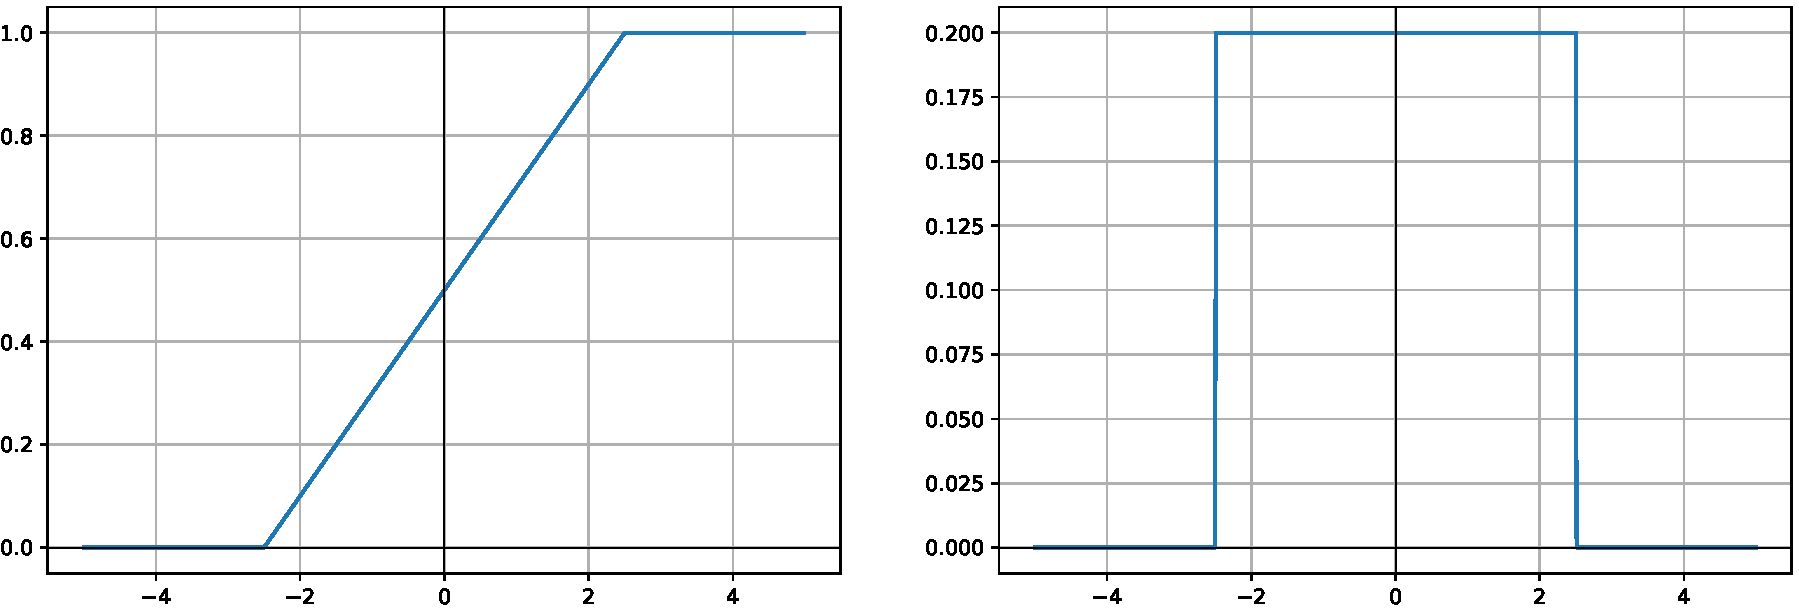
\includegraphics[width=\textwidth]{Hard_sigmoid.pdf}
\centering
\caption{Tvrda sigmoida i njena derivacija}
\label{fig:hard_sigmoid}
\end{figure}

\begin{equation}
\begin{split}
f(x) = min(1,\ max(0,\ 0.2x + 0.5))
\end{split}
\qquad
\begin{split}
f'(x) = 
\begin{cases}
0.2,	 		& \text{ako } x \in [-2.5, 2.5] \\
0,	& \text{inače}
\end{cases}
\end{split}
\end{equation}

\todo{koji problem rješava}
\todo{svojstva}
\todo{problemi}

\subsection*{Swish}

\begin{figure}[H]
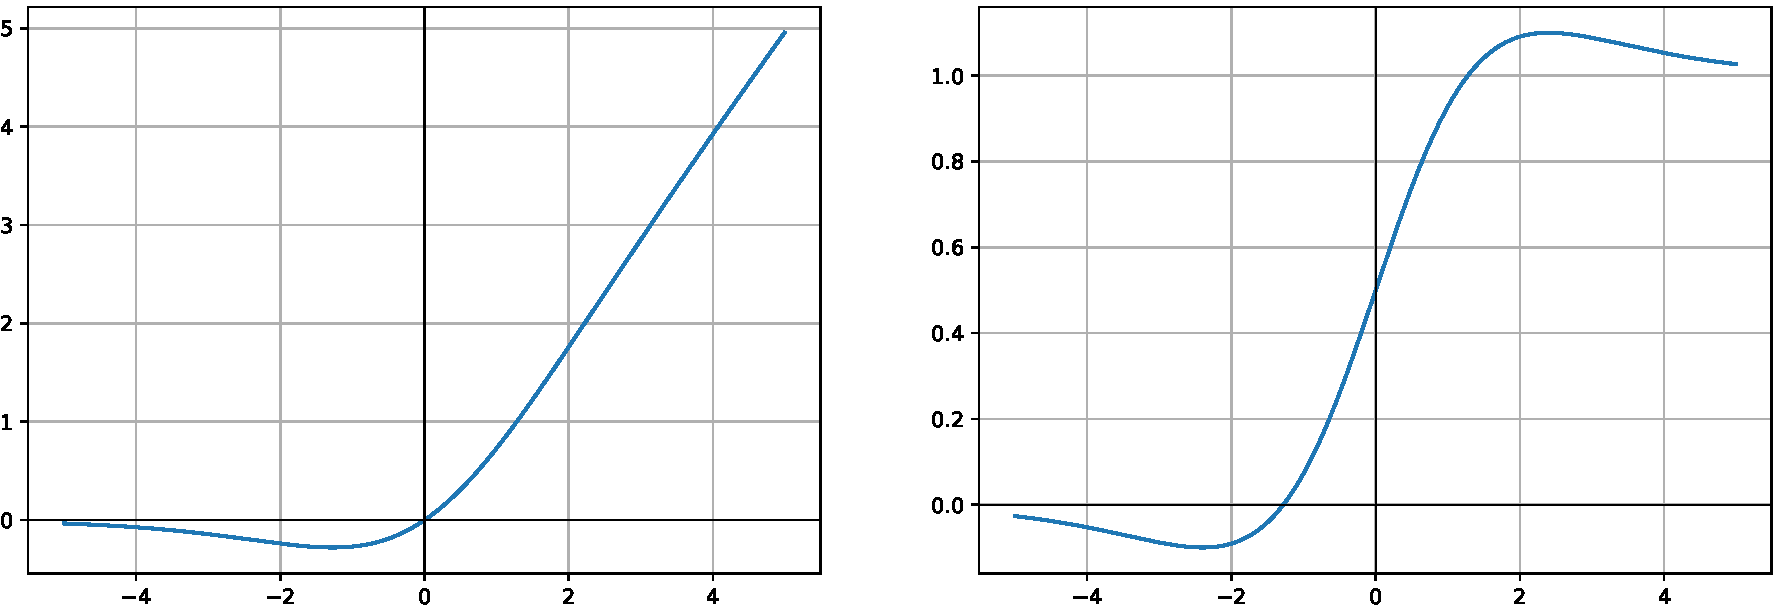
\includegraphics[width=\textwidth]{Swish.pdf}
\centering
\caption{Funkcija Swish i njena derivacija}
\label{fig:swish}
\end{figure}

\begin{equation}
\begin{split}
f(x) = x \sigma(\beta x)
\end{split}
\qquad
\begin{split}
f'(x) &= \sigma(\beta x) + \beta x \cdot \sigma(\beta x)(1-\sigma(\beta x)) \\
&= \frac{e^x \cdot (e^x + x + 1)}{(e^x + 1)^2}
\end{split}
\end{equation}

\todo{koji problem rješava}
\todo{svojstva}
\todo{problemi}

\subsection*{Tangens hiperbolni (tanh)}

\begin{figure}[H]
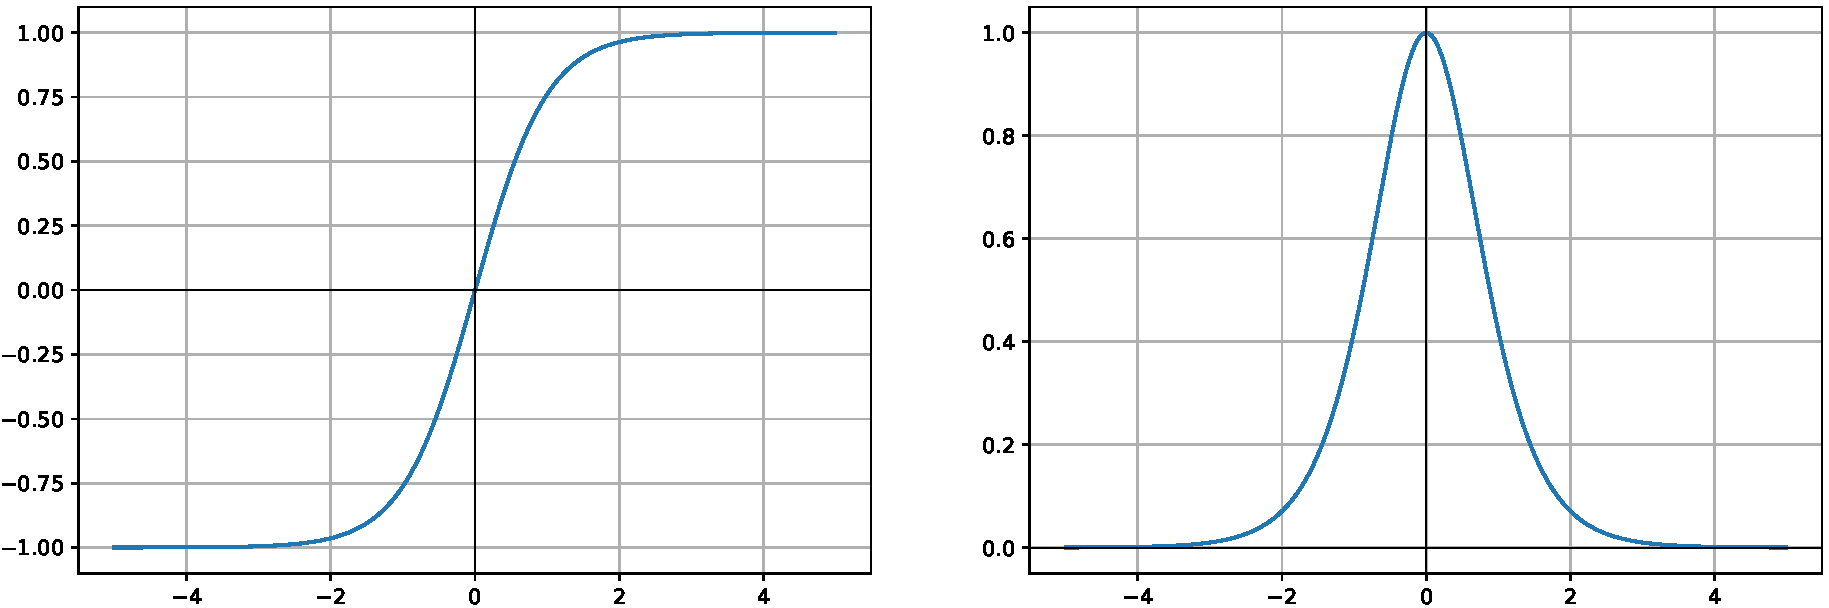
\includegraphics[width=\textwidth]{tanh.pdf}
\centering
\caption{Funkcija tanh i njena derivacija}
\label{fig:tanh}
\end{figure}

\begin{equation}
\begin{split}
f(x) = \frac{e^x - e^{-x}}{e^x + e^{-x}}
\end{split}
\qquad
\begin{split}
f'(x) = 1 - tanh^2(x)
\end{split}
\end{equation}

\todo{koji problem rješava}
\todo{svojstva}
\todo{problemi}

\subsection*{Tvrdi tangens hiperbolni}
\engl{Hard tanh}

\begin{figure}[H]
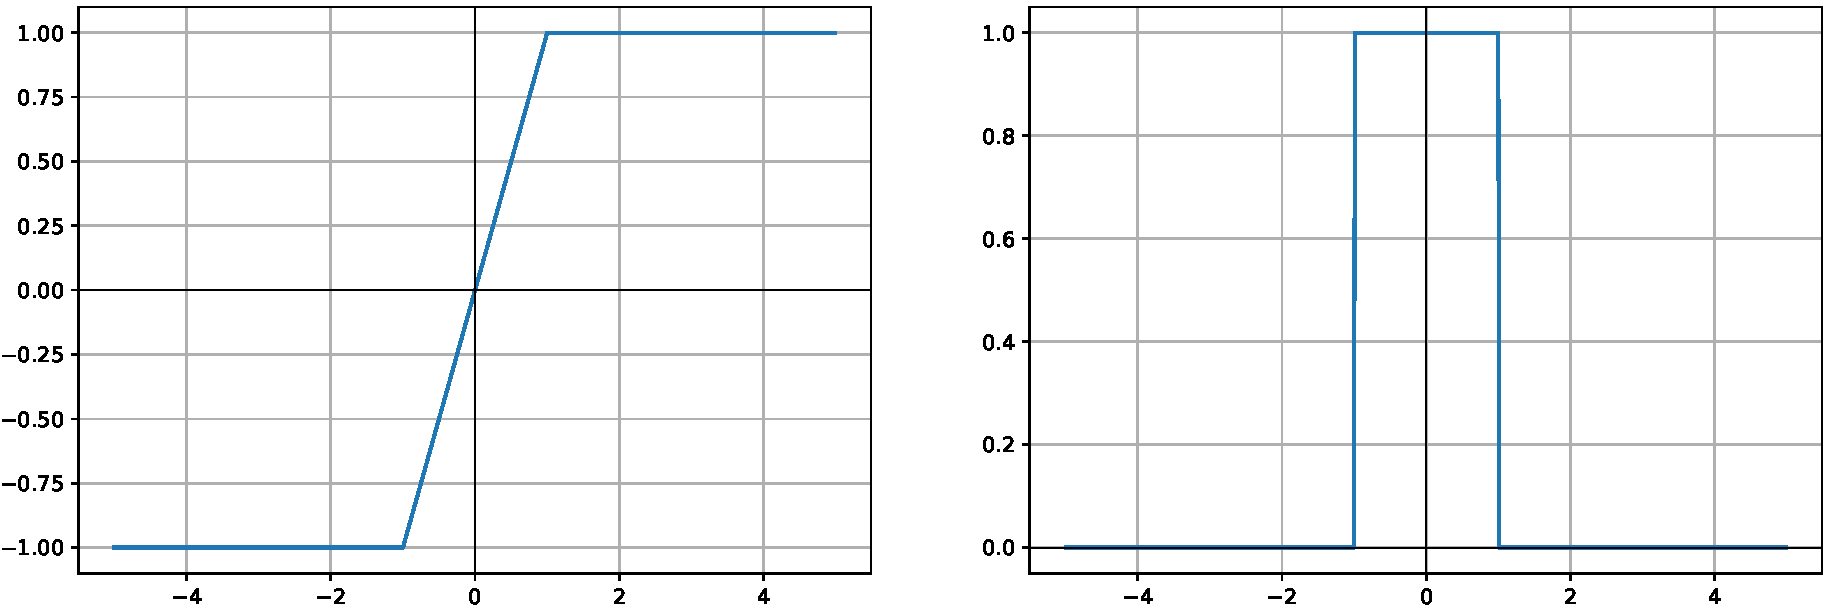
\includegraphics[width=\textwidth]{Hard_tanh.pdf}
\centering
\caption{Tvrdi tanh i njegova derivacija}
\label{fig:hard_tanh}
\end{figure}

\begin{equation}
\begin{split}
f(x) =
\begin{cases}
-1,	 		& \text{ako } x < 1 \\
x,	 		& \text{ako } x \in [-1,1] \\
1,	& \text{inače}
\end{cases}
\end{split}
\qquad
\begin{split}
f'(x) =
\begin{cases}
0,	 		& \text{ako } x < 1 \\
1,	 		& \text{ako } x \in [-1,1] \\
0,	& \text{inače}
\end{cases}
\end{split}
\end{equation}

\todo{koji problem rješava}
\todo{svojstva}
\todo{problemi}

\subsection*{Racionalna aproksimacija tanh}
\engl{Rational tanh}

\todo{DL4J ima bug u derivaciji ove fje}

\todoimg{}

\todo{koji problem rješava}
\todo{svojstva}
\todo{problemi}

\begin{equation}
f(x) = 1.7159 \cdot tanh(\frac{2}{3}x)\text{,\quad gdje }
tanh(x) \approx sgn(x)(1 - \frac{1}{1 + |x| + x^2 + 1.41645 \cdot x^4}) \\
f'(x) =
\end{equation}

\todo{koji problem rješava}
\todo{svojstva}
\todo{problemi}

\subsection*{Ispravljeni tanh}
\engl{Rectified tanh}

\todoimg{}

\todo{koji problem rješava}
\todo{svojstva}
\todo{problemi}

\subsection*{Softmax}

\todoimg{}

\begin{equation}
\begin{split}
f(\vec{x}) = \frac{e^{\vec{x}}}{\sum_ie^{\vec{x_i}}}
\end{split}
\qquad
\begin{split}
f'(x) = \frac{e^x}{1+e^x}
\end{split}
\end{equation}

\todo{koji problem rješava}
\todo{svojstva}
\todo{problemi}

\subsection*{Hierarchical softmax}

\todoimg{}

\begin{equation}
???
\end{equation}

\todo{koji problem rješava}
\todo{svojstva}
\todo{problemi}


\subsection*{Maxout}

\todoimg{}

\begin{equation}
\begin{split}
f(\vec{x}) = 
\end{split}
\qquad
\begin{split}
f'(x) = 
\end{split}
\end{equation}

\todo{koji problem rješava}
\todo{svojstva}
\todo{problemi}

\subsection*{Softplus}

\todoimg{}

\begin{equation}
\begin{split}
f(x) = log(1+e^x)
\end{split}
\qquad
\begin{split}
f'(x) = \frac{e^x}{1+e^x}
\end{split}
\end{equation}

\todo{koji problem rješava}
\todo{svojstva}
\todo{problemi}

\subsection*{Noisy softplus}

\todoimg{}

\begin{equation}
???
\end{equation}

\todo{koji problem rješava}
\todo{svojstva}
\todo{problemi}

\subsection*{Softsign}

\todoimg{}

\begin{equation}
\begin{split}
f(x) = \frac{x}{1+|x|}
\end{split}
\qquad
\begin{split}
f'(x) = \frac{1}{(1+|x|)^2}
\end{split}
\end{equation}

\todo{koji problem rješava}
\todo{svojstva}
\todo{problemi}

\subsection*{Sinus (sin)}

\todoimg{}

\begin{equation}
\begin{split}
f(x) = sin(x)
\end{split}
\qquad
\begin{split}
f'(x) = cos(x)
\end{split}
\end{equation}

\todo{koji problem rješava}
\todo{svojstva}
\todo{problemi}

\subsection*{Kosinus (cos)}

\todoimg{}

\begin{equation}
\begin{split}
f(x) = cos(x)
\end{split}
\qquad
\begin{split}
f'(x) = -sin(x)
\end{split}
\end{equation}

\todo{koji problem rješava}
\todo{svojstva}
\todo{problemi}

\subsection*{Parabola $x^2$}

\todoimg{}

\begin{equation}
\begin{split}
f(x) = x^2
\end{split}
\qquad
\begin{split}
f'(x) = 2x
\end{split}
\end{equation}

\todo{koji problem rješava}
\todo{svojstva}
\todo{problemi}

\subsection*{Kubna parabola $x^3$}

\todoimg{}

\begin{equation}
\begin{split}
f(x) = x^3
\end{split}
\qquad
\begin{split}
f'(x) = 3x^2
\end{split}
\end{equation}

\todo{koji problem rješava}
\todo{svojstva}
\todo{problemi}

\subsection*{Gauss}

\todoimg{}

\begin{equation}
\begin{split}
f(x) = e^{-x^2}
\end{split}
\qquad
\begin{split}
f'(x) = -2x \cdot f(x)
\end{split}
\end{equation}

\todo{koji problem rješava}
\todo{svojstva}
\todo{problemi}

%--------------------------------------------------------------------------------------%
\chapter{Optimizacija simboličkom regresijom (tehnički genetskim programiranjem...)}

\section{Simbolička regresija}
\todo{Opis i svojstva SR}
\todo{Utjecaj i brojnost parametara u GA (moš linkat i svoj završni rad :P)}

\section{Taboo evolucijski algoritam}
\todo{Problem konvergencije i stohastičnosti GP-a}
\todo{EA oplemenjen taboo listom iz algoritma Taboo pretraživanja}

\section{Korišteni čvorovi (prostor pretraživanja)}
U nastavku je dan popis čvorova koji ujedno definiraju prostor pretraživanja.

\begin{table}
\begin{tabular}[t]{lr}
\begin{tabular}[t]{l|c|r}
\textbf{Naziv} & \textbf{Funkcija} & \textbf{Broj ulaza} \\
\hline
x		& $x$					& 0 \\
const	& $c \in \realnum$		& 0 \\
\hline
+		& $x + y$				& 2 \\
-		& $x - y$				& 2 \\
*		& $x \cdot y$			& 2 \\
/		& $\frac{x}{y + 1e-12}$	& 2 \\
\hline
min		& $min(x, y)$			& 2 \\
max		& $max(x, y)$			& 2 \\
abs		& $|x|$					& 1 \\
\hline
sin		& $sin(x)$				& 1 \\
cos		& $cos(x)$				& 1 \\
tan		& $tan(x)$				& 1 \\
\hline
exp		& $e^x$					& 1 \\
log		& $log_e(x)$				& 1 \\
pow2		& $x^2$					& 1 \\
pow3		& $x^3$					& 1 \\
pow		& $x^y$					& 2 \\
\end{tabular}
& \quad
\begin{tabular}[t]{l|c|r}
\textbf{Naziv} & \textbf{Funkcija} & \textbf{Broj ulaza} \\
\hline
elu		& $ELU(x)$				& 1 \\
gauss	& $e^{x^2}$				& 1 \\
lrelu	& $LReLU(x)$				& 1 \\
relu		& $ReLU(x)$				& 1 \\
selu		& $SELU(x)$				& 1 \\
sigmoid	& $\frac{1}{1+e^{-x}}$	& 1 \\
softmax	& $Softmax(x)$			& 1 \\
sotplus	& $Softplus(x)$			& 1 \\
softsign	& $Softsign(x)$			& 1 \\
swish	& $Swish(x)$				& 1 \\
tanh		& $tanh(x)$				& 1 \\
\end{tabular}
\end{tabular}
\caption{Popis korištenih čvorova}
\end{table}

%--------------------------------------------------------------------------------------%
\chapter{Implementacija}
\section{Razvojna okolina i alati}
\todo{tulavi DL4J}
\todo{IntelliJ <3 <3 <3}
\todo{funkcije iscrtavam u jn}

\section{Parametri}
\todo{da, možeš definirat parametre u datoteki}
\todo{dodavanje parametara}
\todo{grid search mehanizam}

\section{Evolucijski algoritmi}
\todo{in-house EA okolina}
\todo{glavne komponente koda}
\todoimg{IntelliJ generirna UML paketa genetics}

\section{Neuronske mreže}
\todo{glavne komponente}
\todo{automatizirana pohrana rezultata}
\todoimg{IntelliJ generirna UML paketa neurology}

\section{Paralelizacija}
\todo{workarbiter <3}
\todo{sinkronizacija u GA i pomoćne klase/metode}

\section{Loggovi}
\todo{kaj sve imaš i kak se koristi}

%--------------------------------------------------------------------------------------%
\chapter{Rezultati}

\section{9class}

\subsection{Uobičajene izlazne funkcije}
\todo{Opis postupka pretrage}
\todo{Tablica}
\todo{Komentar}

\subsection{Utjecaj parametra veličine taboo liste}
\todo{Tablica}
\todo{Komentar}

\todoimg{boxplot}

\section{256class}

\subsection{Uobičajene izlazne funkcije}
\todo{Opis postupka pretrage}
\todo{Tablica}
\todo{Komentar}

\subsection{Utjecaj parametra veličine taboo liste}
\todo{Tablica}
\todo{Komentar}

\todoimg{boxplot}

%--------------------------------------------------------------------------------------%
\chapter{Stvari koje sam probao, ali nisu ispale korisne}
\subsubsection{Učeći parametri}
\todo{dokaz da na korištene funkcije nema utjecaja (stopi se s težinama ili biasom)}
\todo{pokazati primjer fje gdje bi se mogao koristiti}

\subsubsection{Dropout}
\todo{zahtjeva previše iteracija, što nije baš korisno u EA okruženju}
\todo{probati maxout?}

\subsubsection{Tensorflow Java API}
\todo{probo, ali je još u razvoju (puno toga je falilo)}

%--------------------------------------------------------------------------------------%
\chapter{Buduća istraživanja}
\todo{Primjena CNN na vremenskim uzorcima po uzoru na onaj rad}
\todo{Ispitivanje učinkovitosti korištene optimizacije na ostalim problemima}
\todo{Paralelna evolucija arhitekture i aktivacijskih fja}

%--------------------------------------------------------------------------------------%
\chapter{Zaključak}
\todo{Radi/Ne radi}
\todo{Pronađene zanimljivosti}
\todo{Pouka za doma}

\bibliography{literatura}
\bibliographystyle{fer}

\begin{sazetak}
Proučiti postojeće metode u izgradnji izlaznih funkcija u umjetnim neuronskim mrežama. Posebnu pažnju posvetiti evolucijskim algoritmima simboličke regresije za izgradnju ciljanih funkcija. Ustanoviti moguće nedostatke postojećih algoritama ili mogućnost poboljšanja. Primijeniti evoluirane izlazne funkcije u homogenoj ili heterogenoj umjetnoj neuronskoj mreži na skupovima DPAv2 i DPAv4 te odrediti mjere kvalitete izgrađenog klasifikatora: točnost, preciznost, odziv te F mjere. Usporediti učinkovitost ostvarenih postupaka s postojećim rješenjima iz literature. Radu priložiti izvorne tekstove programa, dobivene rezultate uz potrebna objašnjenja i korištenu literaturu.

\kljucnerijeci{Ključne riječi, odvojene zarezima.}
\end{sazetak}

\engtitle{Optimized output functions for classifiers based on artificial neural networks in the domain of implementation attacks on cryptographic devices}
\begin{abstract}
Examine existing methods in building output functions in artificial neural networks. Give special attention to evolutionary algorithms of symbolic regression for constructing target functions. Apply evolved output functions in a homogeneous or heterogeneous artificial neural network on datasets DPAv2 and DPAv4 and examine quality measures of the built classifier: accuracy, precision, recall and F measures. Compare the efficiency of acquired methods with existing solutions from the literature. Alongside thesis attach source code of programs, acquired results with necessarry discussion and literature used.

\keywords{Keywords.}
\end{abstract}

\end{document}
